\chapter{DAH Projects}
\label{sec:projects}


\section{Project B: Building an FFT Spectrum Analyser}

\subsection{Goals of project}

You will develop and build a real-time spectrum analyser. This device will sample an analog signal and perform a Fast Fourier Transform (FFT) analysis and the results can be displayed and/or written to a file. The ADC MC3208 chip, which was used during the checkpoints,  could be a part of this project. 

The projects have an open-ended aspect and are an opportunity where you can show your own initiative and demonstrate your experimental and computational skills. 


\subsection{Equipment for project B}

For this project you will need the following items:
\begin{itemize} 
\item Raspberry-Pi
\item Signal generator
\item Analog to Digital Converter (MCP3208)
\item Arduino Uno 
\item USB cable to connect Arduino to Raspberry-Pi.
\item Microphone with preamplifier if you want to analyse acoustic signals. 
\end{itemize}
Some of this equipment will be located in the red box B. You will have to share some items between Tuesday and Thursday sessions. 


\subsection{Building the FFT spectrum analyser}

We suggest that you start by reading up on Fourier transformations, which you learned in a 3rd year course, and the Fast Fourier Transform as a particularly effective numerical implementation. You may also want to familiarise yourself with the Arduino micro controller, e.g. at \url{http://www.arduino.cc/}. It is suggested to develop and build the spectrum analyser in a modular way, e.g. to develop the FFT analysis separately from the real-time data acquisition, before combining these tasks.

There are many ways of completing this project. To give you a better idea of what may be required, take a look at the three examples below, listed in the order of increasing complexity. 

\begin{enumerate}
\item	Use the \webiopi framework. This is the simplest approach because it requires almost no new knowledge. You would use the signal generator to produce a waveform and connect the ADC (MC3208) chip to the Raspberry-PI using the SPI interface. Use the ADC chip (MCP3208) to sample the signal at regular intervals, fill an array of a fixed length (say, 1024 samples) and perform an FFT analysis of the data using a Numpy library (routine  \begin{tt}numpy.fft.rfft()\end{tt}).
 You would then save the absolute values of the FFT data to file and display these on a screen. This task would allow you to develop the FFT analysis and the displays. The amount of work for this is similar to a checkpoint. 

While such an FFT analyser is simple to build and control, it has severe limitations. \webiopi allows only for a very low sampling rate (as studied in Checkpoint 3). There can be missing parts in the recorded samples ("data holes") as the Raspberry-Pi is not a real-time computer. The Raspberry-Pi has a multitasking operating system, which can interrupt the data taking, especially if sampled at too large a rate.

\item Use the MCP3208 ADC chip, but control and read its output directly through the serial interface SPI using a python library called \begin{tt}spidev\end{tt}, which is already installed on the Raspberry-Pi.
%
\begin{comment}
which you will need to install on the Raspberry-Pi:
    pi@Demonstrator-pi ~ $ mkdir spidev 
    pi@Demonstrator-pi ~ $ cd spidev 
    pi@Demonstrator-pi ~ /spidev $ wget https://raw.github.com/doceme/py-   spidev/master/setup.py 
    pi@Demonstrator-pi ~ /spidev $ wget https://raw.github.com/doceme/py-    pi@Demonstrator-pi ~ $spidev/master/spidev_module.c 
    pi@Demonstrator-pi ~ /spidev $ sudo python setup.py install  
\end{comment}
%
The spidev library has a routine called \begin{tt}xfer()\end{tt}  that sends an array of bytes to the ADC through the SPI interface and receives ADC data in response to this request. Use \begin{tt}xfer()\end{tt}   to instruct the ADC to measure the voltage. To read the voltage from CH0 of the ADC one needs to send three bytes [6,0,0] 
which instructs the ADC to select channel CH0, measure the voltage and then send back another three bytes (ignore the first byte, the second and the third are the high and the low byte of the 12-bit integer output of the ADC) to the Raspberry-Pi.

\lstinputlisting{../scripts/project_B_a.py}
 
This method is much faster than \webiopi  and it is possible to record up to 5k samples per second, however real-time sampling is not possible and there can be holes in the data.

\item	Use the Arduino, a real-time \microcontroller, which  is a small computer on a single integrated circuit containing a processor core, memory, and programmable input/output peripherals, 
The Arduino is based on an 8-bit 16MHz chip ATmega328 and does not have an operating system by default, so it supports real-time computing, i.e. the program does not get interrupted. The Arduino also has a built-in 10-bit ADC. For this project, the Arduino is used as an ADC and a data buffer connected to the Raspberry-Pi and it will be made available pre-programmed. From your perspective the Arduino will behave as "black box", i.e. an ADC with a buffer memory that can be accessed through an USB interface. (Note: If you are interested, you may familiarise yourself with Arduino-IDE package and upload the code, {\tt ADCforRPI4.ino},  available on  \url{https://github.com/fmuheim/DAH}. 
You will need to write python code that communicates with the Arduino using the \begin{tt}serial\end{tt} library.\\

\lstinputlisting{../scripts/project_B_b.py}

 The 8-bit resolution simplifies data transfer and processing, since each sample equals exactly one byte of data. In fact, 8 bits correspond to the effective resolution of the ADC at the largest supported sampling frequencies where the two least significant bits (of the 10-bit ADC) are essentially noise,
This method allows for fast sampling rates of up to 100k samples per second in real-time and there are no data holes.
\end{enumerate}

\subsection{Performing an FFT spectrum analysis}

Performing an FFT analysis a data sample is straightforward, for example you can use a Numpy library routine, \begin{tt}numpy.fft.rfft()\end{tt}. In all cases the data should be saved to a file and displayed on the screen.  Once the FFT spectrum analyser is working and the main functionalities for saving and displaying the data spectrum is achieved, there are several possibilities to take this project forward in an open-ended way. 

\begin{enumerate}

\item	You will use FFT to analyse the spectrum of a several repetitive signal shapes, including a sinusoidal, a square and a saw waveform generated by the function generator, and compare the amplitudes of different harmonics to mathematically predicted ones for that signal.

\item Investigate which of the many python libraries that are available for drawing on the screen best suits your needs. For example, mathplotlib can be employed to produce high-quality figures, but may be too slow to present data in real time. The \begin{tt}pygame\end{tt} library supports drawing simple figures (points, lines, etc.) and is very fast, simple to use, and sufficient for making simple plots of the input signals and its FFT spectrum.

\item There are additional methods for generating signals. For example you can use a microphone to record acoustic signals and perform FFT analyses on these samples. Can you use it e.g. to determine the pitch of a whistled note?

\item The Arduino is used as a "black box" for this project. Learning how to program was deemed to be incompatible with the timescale of the project. However, if you have used the Arduino before or are sufficiently curious, you are welcome to investigate. There might be also other options for reading the data, and you are encouraged to investigate this.

\end{enumerate}

\subsection{Project planning}

The project descriptions are generally significantly less detailed than what was made available for the checkpoints. Any material covered during checkpoints including python code examples are assumed to be known.  Only essential and new information is provided and you are expected to take care of the details. Python code snippets are provided where necessary, but you will have to understand yourself what they do. It is recommend that you google for information about your project on the web, including data sheets of components and python libraries, if applicable. Python scripts should be well structured, either using functions or classes.

The timeline will vary between different projects, but in general, it is recommended that you plan your work as follows:
\begin{itemize}
\item	weeks 7, 8 \& 9: 	Building your gadget and/or writing code for project;
\item	week 9, 10: 	Analysis of data or equivalent, prepare supplementary material;
\item	week 10, 11:	Finish writing of project report and prepare submission.
\end{itemize}
Note that you are advised to start writing your report as the project progresses. 

For guidance on report writing, how the projects will be assessed, plagiarism and the submission deadline, please consult the DAH course booklet and the DAH grade descriptors, available on Learn.



\newpage
\section{Project C: Building a Synthesizer}

\subsection{Goals of project}

You will develop and build a small synthesizer with which you will be able to play small tunes. This project builds upon the work carried out in checkpoint 4 where you worked with an I/O expander chip. With the synthesizer you will be able to play simple tunes, but there is scope for developing the synthesizer much further.

The projects have an open-ended aspect and are an opportunity where you can show your own initiative and demonstrate your experimental and computational skills. 


\subsection{Equipment for project C}

For this project you will need the following items:
\begin{itemize}
\item Raspberry-Pi
\item  Amplified Speakers
\item MCP23S17 IO Expender
\item 1K Resistors
\item Pushbuttons
\end{itemize}
Some of this equipment will be located in the red box C. You will have to share some items between Tuesday and Thursday sessions. 


\subsection{Building the synthesizer}

The SPI I/O expander chip (MCP23S17) is supported by the \webiopi framework. In checkpoint Pi 3 you used an 8 bit I2C expander chip in a very similar way, so you can built upon this work. For this project we recommend that you use the MCP23S17 chip, which is a 16 bit SPI expander. While the
two expander chips are different devices the same python methods can be applied when using \webiopi.
 
\begin{enumerate}
\item Start your project using switch buttons to play sounds at first and then change to free wires forming touch sensors. The insulation from the end of each wire should be stripped. To be able to use the expander chip with wires as touch sensors one should utilise the positive logic (logic 1 means wire was touched).

\item You can base your project on the \begin{tt}Snack\end{tt}  audio package, which is already installed on the Raspberry-Pi. You can find a description on the following Webpage: \url{https://www.daniweb.com/software-development/python/code/216655/play-a-musical-note-python}.
%
Here is an example code of how to use this package.\\

\lstinputlisting{../scripts/project_C_a.py}
\vspace*{-0.5cm}
\end{enumerate}

Once you have set up the hardware, play a few notes and make sure you understand how the synthesizer works. In Appendix 1 of project C, shown below, you can find the frequencies for musical notes.


\subsection{Applications using the synthesizer}

\begin{enumerate}
\item	You can play a tune and record it.

%\item  You may want to try another sound library/package available for python. If you find such a %package ask a demonstrators help to install the package for you on the Raspberry-Pi.

\item There are many ways to enrich your project, for example, try to implement what is called "polyphony" in the world of music synthesizers.

Polyphony means that the synthesizer can play more than one note at the same time, i.e. this means that the synthesizer is able to detect two or more buttons being pressed at the same time. In reality the sound device (i.e. the sound chip of the Raspberry Pi) is producing multiple interleaving sounds, but our hearing sense perceives them as concurrently played sounds.

\item To play two or more sounds at the same time it is not recommended to use the \begin{tt}Snack\end{tt} audio package. Instead you are encouraged to use pre-recorded audio samples from a piano in mp3 format. 

You can download a compressed file with the audio samples from the DAH DropBox page. To play an audio file (sampled note) 
you can use an application such as \begin{tt}mpg321\end{tt} or  \begin{tt}omxplayer\end{tt}. Below an example is given of how to play two sounds at the same time.
Note the \begin{tt}-q\end{tt} command to \begin{tt}mpg321\end{tt}, which stops it from producing unhelpful text output.\\

\lstinputlisting{../scripts/project_C_b.py}
\vspace*{-0.5cm}
\end{enumerate}

Capturing two or more buttons being pressed at the same time can be achieved by reading the expander as a parallel bus instead of reading the state of each push button switch in sequence. (Reading in sequence is commonly referred to as polling). When using parallel or port reading, one should save the state of the port to a variable, which can be called a "switch register". Playing the synthesizer will correspond to sweeping all bits of the switch register for finding pressed switches. After the sweep, one should set the state of the switch register to idle.
 
Can you find where the bottle-neck occurs in trying to achieve polyphony? Is the limitation due to hardware or software?


\subsection{Project planning}

The project descriptions are generally significantly less detailed than what was made available for the checkpoints. Any material covered during checkpoints including python code examples are assumed to be known.  Only essential and new information is provided and you are expected to take care of the details. Python code snippets are provided where necessary, but you will have to understand yourself what they do. It is recommend that you google for information about your project on the web, including data sheets of components and python libraries, if applicable. Python scripts should be well structured, either using functions or classes.

The timeline will vary between different projects, but in general, it is recommended that you plan your work as follows:
\begin{itemize}
\item	weeks 7, 8 \& 9: 	Building your gadget and/or writing code for project;
\item	week 9, 10: 	Analysis of data or equivalent, prepare supplementary material;
\item	week 10, 11:	Finish writing of project report and prepare submission.
\end{itemize}
Note that you are advised to start writing your report as the project progresses. 

For guidance on report writing, how the projects will be assessed, plagiarism and the submission deadline, please consult the DAH course booklet and the DAH grade descriptors, available on Learn.


\vfill

\subsection*{Appendix 1 of Project C: Frequency Table for Notes}
\vspace*{-1.0cm}
\begin{center}                                        
 {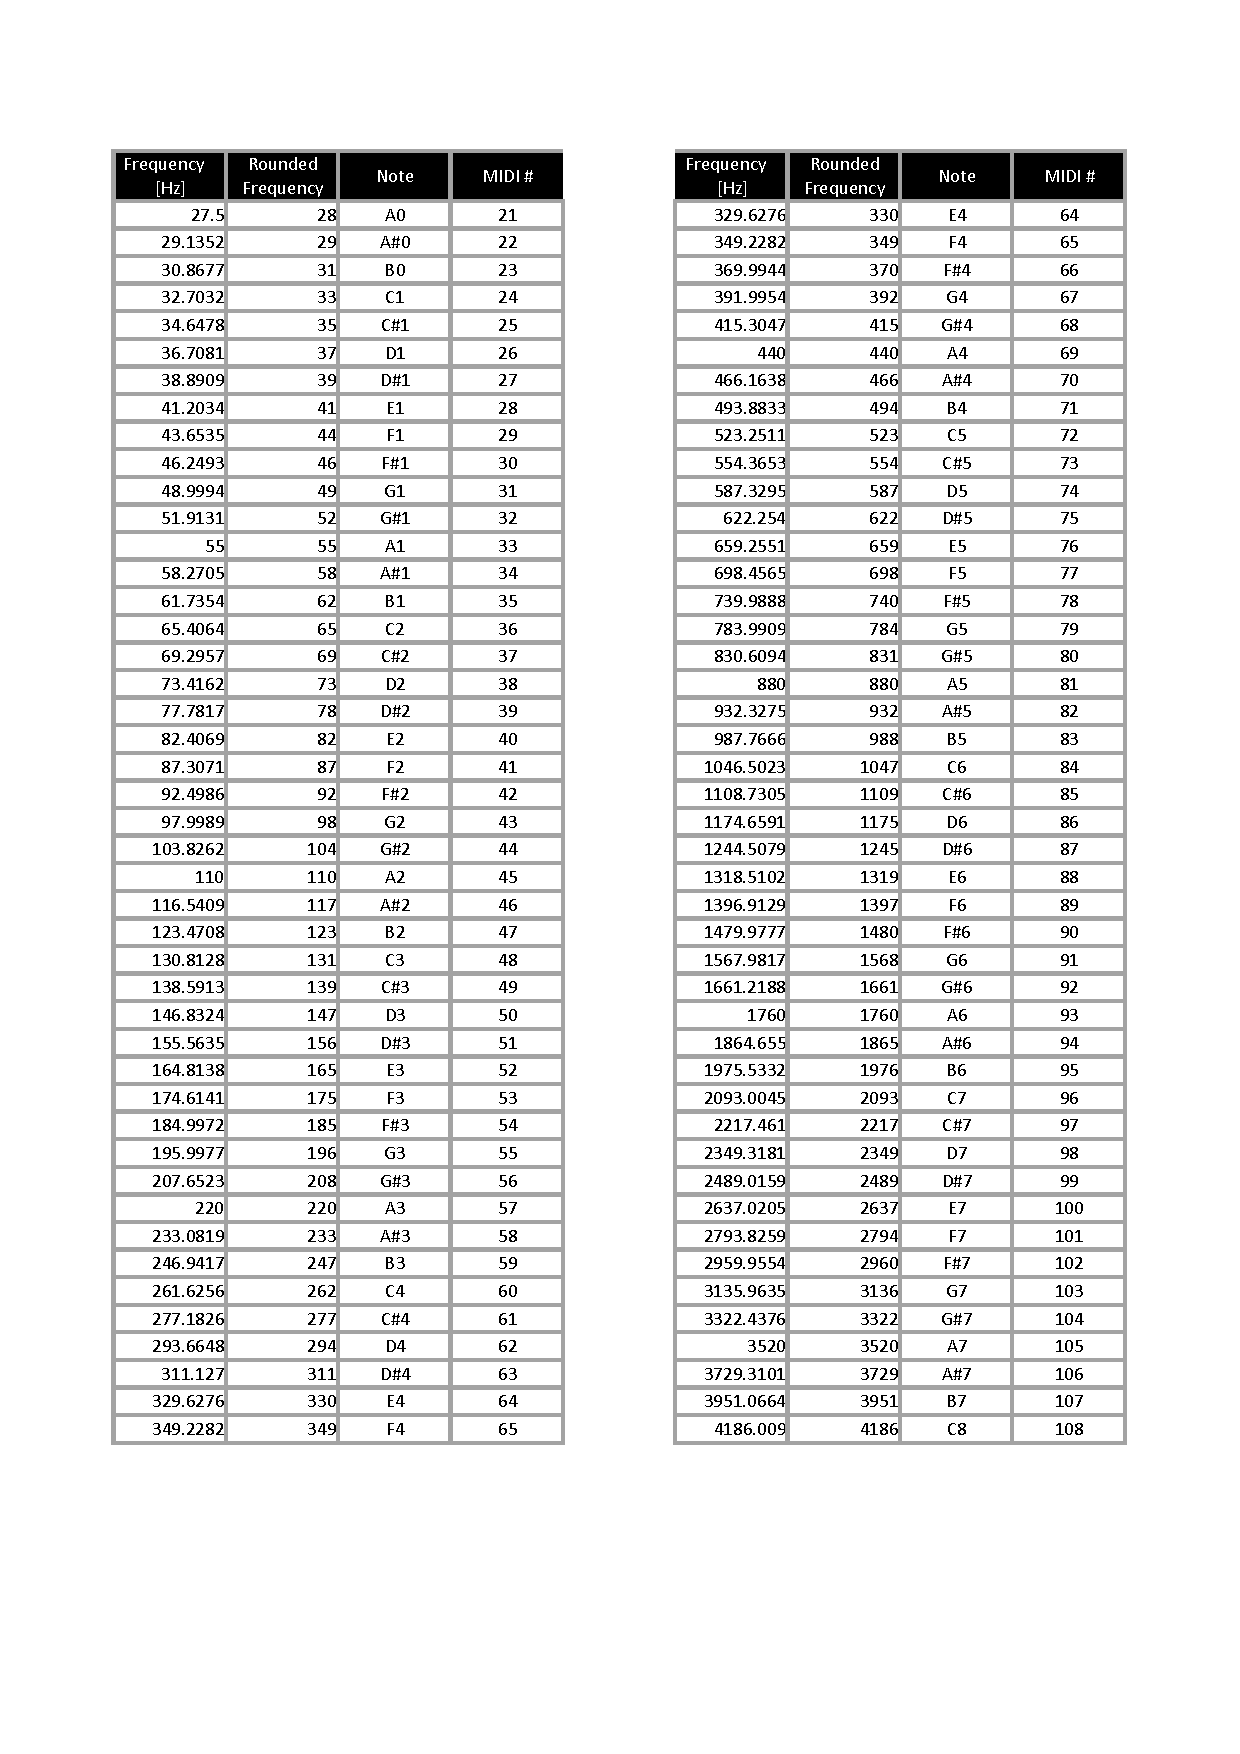
\includegraphics[width=0.90\textwidth]{figs/Frequency-table}}
 \end{center}
 
 
 \newpage
\section{Project D: Building an Ultrasonic Range Finder}

\subsection{Goals of project}

You will develop and build an ultrasonic range finder. This device will use an ultrasound transducer as a distance sensor. 
%The \webiopi framework, which was used during the checkpoints will be a part of this project. 

The projects have an open-ended aspect and are an opportunity where you can show your own initiative and demonstrate your experimental and computational skills. 

\subsection{Equipment for project D}

For this project you will need the following items:
\begin{itemize}
\item Raspberry-Pi
\item Ultrasonic Transducer module HC-SR04
\item 1 k$\Omega$ Resistor
\item Loudspeakers
\end{itemize}
Some of this equipment will be located in the red box D. You will have to share some items between Tuesday and Thursday sessions. 


\subsection{Building the ultrasonic range finder}
 
You will develop an ultrasonic range finder using a HC-SR04 Distance Sensor. 
Start by connecting the HC-SR04 to the Raspberry-Pi, as shown in the Figure below. Test the circuit using the code examples, which are provided in Appendix 1 of project D below. 
%You will need to make changes in your scripts  so that it will work within the \webiopi framework.
You will need to make a few changes in your script  to get it to work.

\begin{center}                                        
 {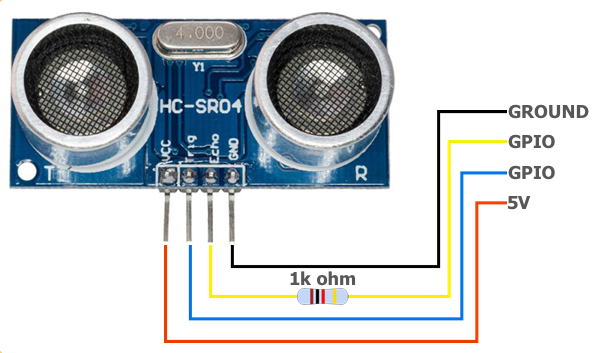
\includegraphics[width=0.50\textwidth]{figs/hcsr04.png}}
 \end{center}


Hints: The output of the HC-SR04 module is a logic level one of 5 V. The Raspberry-Pi works with 3.3V logic signals. A 1 k$\Omega$ resistor in series will limit the current in the circuit to prevent damaging the Raspberry Pi.
 
\begin{enumerate}
\item 	Work out how the HC-SR04 sensor operates. What are the "Trig" and "Echo" pins of the HC-SR04 module used for? Use the oscilloscope to capture these signals when running the code example. 

\item Use these data to explain in detail how the module works and how it is possible to measure distance using ultrasonic waves.

%\item  Rewrite  your scripts using the  \webiopi instead of the \begin{tt}RPi\end{tt} framework.
\item  Familiarise yourself with the  \begin{tt}RPi\end{tt} framework, see e.g. \\
\url{https://sourceforge.net/p/raspberry-gpio-python/wiki/BasicUsage}.\\
Using the \begin{tt}RPi\end{tt} framework complete the function \begin{tt} def reading(sensor):\end{tt} in your script and test your circuit.

\item What are the minimum and maximum distance that your Range Finder can measure? 
\end{enumerate}

\subsection{Applications using the ultrasonic range finder}

Now that you have a functioning ultrasonic range finder there are several possible applications.

\begin{enumerate}

\item	Try to understand better the properties and limitations of your device. What are the minimum and maximum size of objects the range finder is able to detect? Play with reflecting surfaces of different areas and define the angular range (span of angles) within the range finder works? Is this approach suitable for large or small objects? Is there a relation between the distance and the size of the reflection area?

\item Develop an application of your choice. An example could be an electronic "Car Parking Assistant" where sounds are created and LEDs flash (or similar) if the sensor gets too close to an object.

\item Perform a calibration of the distance scale of your application.

\end{enumerate}

Note that the loudspeakers are power hungry, so they  should be connected  via USB to the 
monitor.

To play an audio file (sampled note) you can use an application such as \begin{tt}mpg321\end{tt} or or  \begin{tt}omxplayer\end{tt}. Below an example is given of how to play a note using a python script.\\

\lstinputlisting{../scripts/project_D_a.py}
\vspace*{-0.5cm}


\subsection{Project planning}

The project descriptions are generally significantly less detailed than what was made available for the checkpoints. Any material covered during checkpoints including python code examples are assumed to be known.  Only essential and new information is provided and you are expected to take care of the details. Python code snippets are provided where necessary, but you will have to understand yourself what they do. It is recommend that you google for information about your project on the web, including data sheets of components and python libraries, if applicable. Python scripts should be well structured, either using functions or classes.

The timeline will vary between different projects, but in general, it is recommended that you plan your work as follows:
\begin{itemize}
\item	weeks 7, 8 \& 9: 	Building your gadget and/or writing code for project;
\item	week 9, 10: 	Analysis of data or equivalent, prepare supplementary material;
\item	week 10, 11:	Finish writing of project report and prepare submission.
\end{itemize}
Note that you are advised to start writing your report as the project progresses. 

For guidance on report writing, how the projects will be assessed, plagiarism and the submission deadline, please consult the DAH course booklet and the DAH grade descriptors, available on Learn.




\subsection*{Appendix 1 of project D: Example Code}

\lstinputlisting{../scripts/project_D_b.py}


\newpage
\section{Project E: Building a Precision Refrigerator}

\subsection{Goals of project}

The course organiser would like to celebrate the DAH course with a glass of fine wine, chilled to exactly the right temperature.
You will design and build a thermostat to precisely control the temperature of a fluid.
Regrettably, fine wine could not be made available for teaching purposes and it will be replaced by a beaker of tap water for this project.
You will use a Peltier thermoelectric device to cool the liquid.
The temperature of the liquid will be monitored using 1-wire temperature sensors, which were used during the checkpoints.

The projects have an open-ended aspect and are an opportunity where you can show your own initiative and demonstrate your experimental and computational skills. 

\subsection{Equipment for project E}

For this project you will need the following items:
\begin{itemize}
\item Raspberry-Pi
\item DC power supply
\item Peltier thermoelectric device
\item 2x temperature sensor S18B20
\item Power transistor Darlington TO-220
\item Heat sinks
\item Beaker
\end{itemize}
Some of this equipment will be located in the red box E. You will have to share some items between Tuesday and Thursday sessions. 


\subsection{Building the refrigerator}

You will need to build a circuit to supply power to the Peltier element as the Raspberry-Pi cannot supply enough current itself.
You can use the power supplies available in the lab, to produce a DC voltage and control it using a power transistor connected to a GPIO pin on the Raspberry-Pi.
Use a 1\,A, 1\,V supply for the Peltier.

\begin{center}
	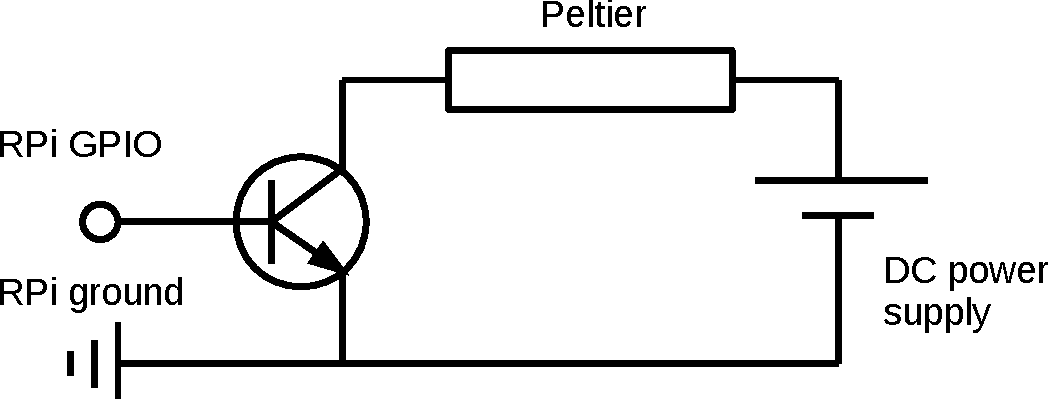
\includegraphics[width=0.5\textwidth]{figs/PeltierCircuit}\\
	%\caption
	{Example circuit diagram for Peltier control.}
\end{center}

Research Peltier devices: note that one side gets hot as the other side gets cold, so you will need to place the hot side in contact with a heat sink.
Do not power the device for more than a few seconds without this heat sink, or you may damage it!
You may also need a heat sink for the transistor.

The temperature of the liquid must be monitored, so you will need to find a way to get the 1-wire sensors near to it.
You will be provided with a waterproof temperature sensor, with part number DS18B20, so you will need to adjust your code appropriately if reading it with \webiopi.

\subsection{Monitoring and controlling the temperature}

Aim first to be able to precisely control the liquid at a few centigrade below room temperature before trying to find out how cold you can make the liquid.
The Peltier device will take a long time to cool the liquid much below room temperature, so don't waste time waiting for this.

During Checkpoint 5 you already learned how to read information from the 1-wire temperature sensors, but you should now consider this in more detail.
How precisely can you measure the temperature of the liquid?
Are there systematic effects that you can account for by calibrating your sensors?
What will you do about temperature gradients across your refrigerator when the Peltier element is switched on?
Remember that you have additional (but not waterproof!) sensors that you used in Checkpoint 5 --- these might be useful, and you have already studied their performance.

Your project should include a way of displaying the current temperature of the liquid, and previous measurements.
You should also include a visual indication of the state of the Peltier, rather than just poking it to see if it feels cold.

The circuit to power and control your Peltier device is simple, but you should think carefully about when your python code should switch the cooling on and off.
Rather than having a simple threshold temperature for turning the cooling on and off, you may want to use a hysteresis loop.
Rapidly toggling power to the Peltier in an uncontrolled fashion is unlikely to give good performance.

You could enhance the scope of your project in the following ways.
\begin{enumerate}
	\item Try varying the cooling power of your Peltier using pulse-width modulation.
		Here you would use your Raspberry Pi GPIO pin to create a square wave to toggle the power transistor on and off.
		You then adjust what percentage of time is spent in the on or off state: the `duty cycle.'
	\item Write an interface that allows the user to start and stop the temperature control programme, show the status and temperature of the Peltier, and change the temperature value of the thermostat.
	\item Consider running the Peltier as a heating element. What changes are required to the sensor, the circuit and the control programs?
\end{enumerate}

\subsection{Project planning}

The project descriptions are generally significantly less detailed than what was made available for the checkpoints. Any material covered during checkpoints including python code examples are assumed to be known.  Only essential and new information is provided and you are expected to take care of the details. Python code snippets are provided where necessary, but you will have to understand yourself what they do. It is recommend that you google for information about your project on the web, including data sheets of components and python libraries, if applicable. Python scripts should be well structured, either using functions or classes.

The timeline will vary between different projects, but in general, it is recommended that you plan your work as follows:
\begin{itemize}
\item	weeks 7, 8 \& 9: 	Building your gadget and/or writing code for project;
\item	week 9, 10: 	Analysis of data or equivalent, prepare supplementary material;
\item	week 10, 11:	Finish writing of project report and prepare submission.
\end{itemize}
Note that you are advised to start writing your report as the project progresses. 

For guidance on report writing, how the projects will be assessed, plagiarism and the submission deadline, please consult the DAH course booklet and the DAH grade descriptors, available on Learn.


 
 
 
\newpage
\section{Project F1: Make Accurate Measurements of Particle Masses}

\subsection{Goals of project}

You will use LHCb data on the invariant mass of particle candidates that you were introduced to during a checkpoint. You will analyse this in a much more sophisticated way and closer to the actual analysis performed leading to its publication. You will use the maximum likelihood process to fit different mass model shapes to the data. From this you will determine the parameters of the mass model for the three signal peaks, and their errors. You will start with a very simple Gaussian mass model. You will then improve this and use a more sophisticated model.

The projects have an open-ended aspect and are an opportunity where you can show your own initiative and demonstrate your experimental and computational skills. 

\subsection{Equipment for project F1}

Note: this is a data analysis project, which does not require use of the Raspberry Pi.
This project is best carried out using the Physics CPlab computers. No other equipment is needed.  There is a CPlab computer available on every desk in the DAH laboratory.
You may also use your own laptop computer, but you will need to be able to install
python and python packages on your own. 


\subsection{Detailed project description}
  
You were previously introduced to the LHCb Upsilon data. 
The LHCb experiment at the Large Hadron Collider at CERN has recorded a sample of muon pairs with invariant masses in the range of 8.5 to 11 GeV/$c^2$. Three clear peaks are observed in this mass spectrum. These correspond to the production of Upsilon mesons, which are bound states of a $b$ and a anti-$b$ quark. These states are known as the $\Upsilon \rm (1S)$, $\Upsilon \rm (2S)$ and $\Upsilon \rm (3S)$ mesons where the $\Upsilon \rm (1S)$ meson is the ground state and the $\Upsilon \rm (2S)$  and $\Upsilon \rm (3S)$  states are radial excitations (for LHCb paper, see {DOI: 10.1007/JHEP06(2013)064).}


During checkpoint 6, you performed some very simple "peak finding". In this project you are going to do the analysis much like it would actually be carried out in a particle physics experiment.

\begin{enumerate}
\item Consider first the Upsilon(1S) ($\Upsilon \rm (1S)$) particle, which is the particle with the lowest mass, i.e. the left most  peak in the plot. Construct a composite probability density function (PDF) for the invariant mass of the muon pairs, which contains two components:
\begin{itemize}
\item A Gaussian shape to fit the  $\Upsilon \rm (1S)$ mass peak;
\item A shallow falling exponential to fit the background shape of the mass spectrum underneath and around the peak.
\end{itemize}

\item	Use this PDF in a Maximum Likelihood fit to determine the parameters of the PDF. Note hat it is essential that the composite PDF remains normalised to 1 over the range of the fit.

Determine the $\Upsilon \rm (1S)$  meson mass and yield, and all other parameters, and their and errors.

You should be able to obtain the parameter errors directly from the minimization engine of your choice (scipy.optimize.minimise, scipy.optimise.curve\_fit, lmfit, see \url{https://lmfit.github.io/lmfit-py/} or Minuit). Depending on your choice you will be able to chose different minimising methods.
It would be good to show that you understand these by obtaining them yourself from the parameters of the Gaussian signal fit - this is described in the data handling lectures.

Plot the fitted signal shape on top of the data.

\item Now consider the entire mass range, and perform a simultaneous fit for all three Upsilon peaks, and the underlying background. Again you should always report the parameter values, and their errors. Plot the fitted signal shape on top of the data.

\item The results so far probably look "quite good" by eye.  i.e. the signal shape plotted on top of the data probably looks like it fits quite well.  However this can be misleading when performing a precision measurement.  You should make a plot of what are called the "residuals". A residual is the difference between the data in the binned histogram and the best-fit mass model value for the centre of that bin. Describe what you see.

\item There are several ways to enhance the scope of the project. For example, if the single Gaussian mass model does not fit the data perfectly, one can try other mass models, i.e. by using a signal PDF that goes beyond a single Gaussian function.  Two examples are:
\item A PDF comprising a function which is the sum of two Gaussian functions (i.e. one narrow and one wide Gaussian function to fit a single Upsilon mass peak)
\item A Crystal Ball function, which incorporates a non-Gaussian tail at the lower end of the mass peak. The functional shape is described elsewhere, e.g. see: \url{http://en.wikipedia.org/wiki/Crystal_Ball_function}. 

You could implement each of these functions in your PDF and see how much better they are at describing the data.

\item Read the publication and see what is said about systematic errors.  Make a reasonable attempt at determining some systematic errors on the masses.

\item As on open ended activity, you will see in the paper that the analysis is also done by dividing the data up into bins of transverse momentum (pT) and rapidity (eta). You can explore doing this analysis yourself. It is somewhat more complex as you have to think about which are common parameters (e.g. masses) and which are not (e.g. background fractions.) Larger dataset, including transverse momentum are available if required.

\end{enumerate}

\subsection{Project planning}

The project descriptions are generally significantly less detailed than what was made available for the checkpoints. Any material covered during checkpoints including python code examples are assumed to be known.  Only essential and new information is provided and you are expected to take care of the details. Python code snippets are provided where necessary, but you will have to understand yourself what they do. It is recommend that you google for information about your project on the web, including data sheets of components and python libraries, if applicable. Python scripts should be well structured, either using functions or classes.

The timeline will vary between different projects, but in general, it is recommended that you plan your work as follows:
\begin{itemize}
\item	weeks 7, 8 \& 9: 	Building your gadget and/or writing code for project;
\item	week 9, 10: 	Analysis of data or equivalent, prepare supplementary material;
\item	week 10, 11:	Finish writing of project report and prepare submission.
\end{itemize}
Note that you are advised to start writing your report as the project progresses. 

For guidance on report writing, how the projects will be assessed, plagiarism and the submission deadline, please consult the DAH course booklet and the DAH grade descriptors, available on Learn.

 
 
 


\newpage
\section{Project F2: Make Accurate Measurements of Particle Masses}

\subsection{Goals of project}

You will use LHCb data on the invariant mass of particle candidates that you were introduced to during a checkpoint. You will analyse this in a much more sophisticated way and closer to the actual analysis performed leading to its publication. You will use the maximum likelihood process to fit different mass model shapes to the data. From this you will determine the parameters of the mass model for the three signal peaks, and their errors. You will start with a very simple Gaussian mass model. You will then improve this and use a more sophisticated model.

The projects have an open-ended aspect and are an opportunity where you can show your own initiative and demonstrate your experimental and computational skills. 

\subsection{Equipment for project F2}

Note: this is a data analysis project, which does not require use of the Raspberry Pi.
This project is best carried out using the Physics CPlab computers. No other equipment is needed.  There is a CPlab computer available on every desk in the DAH laboratory.
You may also use your own laptop computer, but you will need to be able to install
python and python packages on your own. 


\subsection{Detailed project description}
 
 You were previously introduced to the LHCb Upsilon data. In this
project you will explore another LHCb dataset where a pair of
oppositely charged kaons and a pion have been combined. Two clear
peaks are observed in this mass spectrum corresponding to the $D_s^+$
and $D^+$ mesons, see figure below % (Fig.~\ref{fig:dmass}). 
For more information see: {DOI:10.1007/JHEP06(2013)065}. 
 
During checkpoint 6, you performed some very simple "peak finding". In this project you are going to do the analysis much like it would actually be carried out in a particle physics experiment.

%
%\begin{figure}[htb!]
\begin{center}
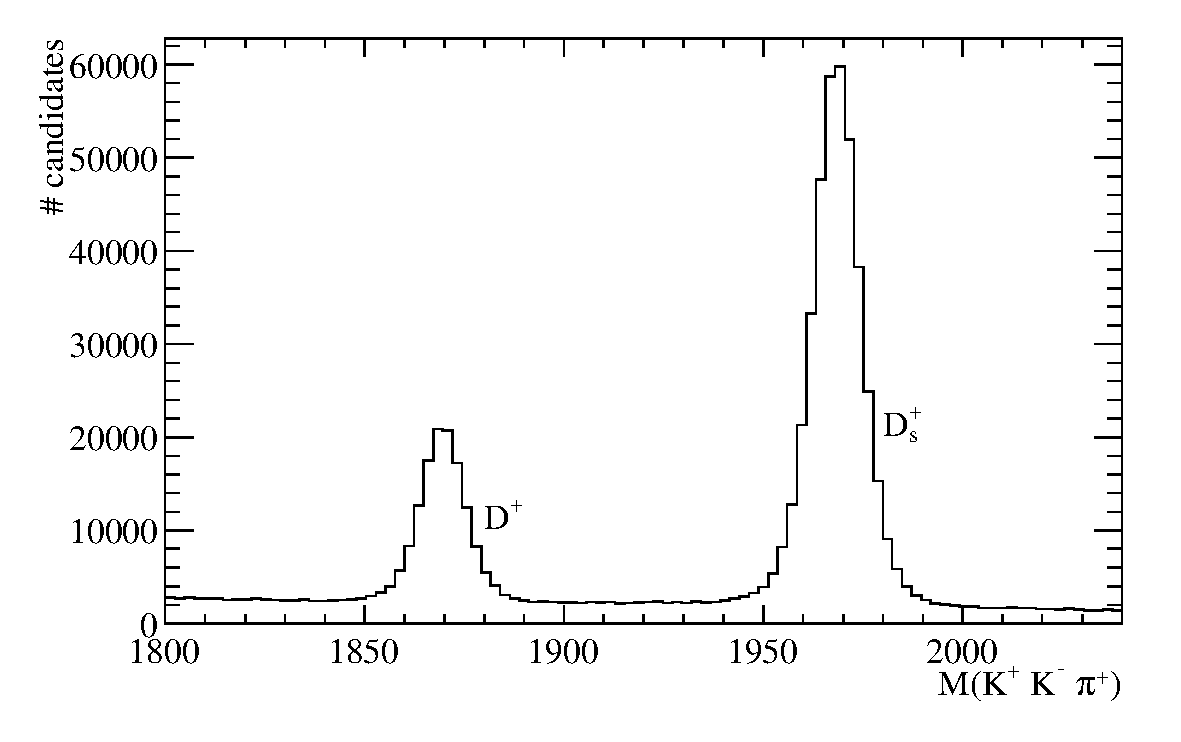
\includegraphics[width=0.75\textwidth]{figs/KKpi.pdf}\\
%\caption
{\small $K^{+}K^{-}\pi^{+}$ invariant mass distribution.}
%\label{fig:dmass}
\end{center}
%\end{figure}
%


\begin{enumerate}

\item Consider first the $D^+$ peak which is the particle with the lowest
mass, i.e. the left most peak in the plot. Construct a composite probability density
function (PDF) for the invariant mass of the muon pairs, which
contains two components : 
\begin{itemize}
\item A Gaussian shape to fit the  $D^+$ mass peak;
\item A shallow falling exponential to fit the background shape of the mass spectrum underneath and around the peak.
\end{itemize}

\item	Use this PDF in a Maximum Likelihood fit to determine the parameters of the PDF. Note hat it is essential that the composite PDF remains normalised to 1 over the range of the fit.

Determine the $D^+$  meson mass and yield, and all other parameters, and their and errors.

You should be able to obtain the parameter errors directly from the minimization engine of your choice (scipy.optimize.minimise, scipy.optimise.curve\_fit, lmfit, see \url{https://lmfit.github.io/lmfit-py/} or Minuit). Depending on your choice you will be able to chose different minimising methods.
It would be good to show that you understand these by obtaining them yourself from the parameters of the Gaussian signal fit - this is described in the data handling lectures.

Plot the fitted signal shape on top of the data.

\item Now consider the entire mass range, and perform a simultaneous fit for both
peaks, and the underlying background. Again you should always report the parameter
values, and their errors. Plot the fitted signal shape on top of the data.
\item The results so far probably look "��quite good"�� by eye. i.e. the signal shape plotted on
top of the data probably looks like it fits quite well. However this can be misleading
when performing a precision measurement. You should make a plot of what are called
the "��residuals"�. A residual is the difference between the data in the binned histogram
and the best-fit mass model value for the centre of that bin. Describe what you see.
\item There are several ways to enhance the scope of the project.

\begin{itemize} 
\item For example, if the single
Gaussian mass model does not fit the data perfectly, one can try other mass models,
i.e. by using a signal PDF that goes beyond a single Gaussian
function. One example: is a PDF comprising a function which is the sum of two Gaussian functions (i.e. one
narrow and one wide Gaussian function to fit a single D meson
peak. Alternatively try a Crystal Ball function, which incorporates a non-Gaussian tail at the lower end of
the mass peak. The functional shape is described elsewhere, e.g. see:
\begin{verbatim}
https://en.wikipedia.org/wiki/Crystal_Ball_function 
\end{verbatim} 
You could implement each of these functions in your PDF and see how much better
they are at describing the data.
\item Read the publication and see what is said about systematic errors. Make a reasonable
attempt at determining some systematic errors on the masses.
\item Compare your results to the PDG and previous measurements.
\item Study how the mass and the width of the peak (the resolution)
  depends on the transverse momentum (pt) and rapidity (eta).
\end{itemize}



\end{enumerate}

\subsection{Project planning}

The project descriptions are generally significantly less detailed than what was made available for the checkpoints. Any material covered during checkpoints including python code examples are assumed to be known.  Only essential and new information is provided and you are expected to take care of the details. Python code snippets are provided where necessary, but you will have to understand yourself what they do. It is recommend that you google for information about your project on the web, including data sheets of components and python libraries, if applicable. Python scripts should be well structured, either using functions or classes.

The timeline will vary between different projects, but in general, it is recommended that you plan your work as follows:
\begin{itemize}
\item	weeks 7, 8 \& 9: 	Building your gadget and/or writing code for project;
\item	week 9, 10: 	Analysis of data or equivalent, prepare supplementary material;
\item	week 10, 11:	Finish writing of project report and prepare submission.
\end{itemize}
Note that you are advised to start writing your report as the project progresses. 

For guidance on report writing, how the projects will be assessed, plagiarism and the submission deadline, please consult the DAH course booklet and the DAH grade descriptors, available on Learn.

 
 


\newpage
\section{Project F3: Make Accurate Measurements of Particle Masses}

\subsection{Goals of project}

You will use LHCb data on the invariant mass of particle candidates that you were introduced to during a checkpoint. You will analyse this in a much more sophisticated way and closer to the actual analysis performed leading to its publication. You will use the maximum likelihood process to fit different mass model shapes to the data. From this you will determine the parameters of the mass model for the three signal peaks, and their errors. You will start with a very simple Gaussian mass model. You will then improve this and use a more sophisticated model.

The projects have an open-ended aspect and are an opportunity where you can show your own initiative and demonstrate your experimental and computational skills. 

\subsection{Equipment for project F3}

Note: this is a data analysis project, which does not require use of the Raspberry Pi.
This project is best carried out using the Physics CPlab computers. No other equipment is needed.  There is a CPlab computer available on every desk in the DAH laboratory.
You may also use your own laptop computer, but you will need to be able to install
python and python packages on your own. 


\subsection{Detailed project description}

You were previously introduced to the LHCb Upsilon data. In this
project you will explore another LHCb dataset where a $\psi(2S)$ meson
(a bound $c\overline{c}$ state) and a pair of
oppositely pions have been combined. Two clear
peaks are observed in this mass spectrum corresponding to the $B_s$
and $B^0$ mesons, see figure below %(Fig.~\ref{fig:bmass}). 
The background shape is quite
complex. At higher masses it is exponential in shape. At lower masses
there is an additional background from the decay $B^0 \rightarrow
\psi(2S) K^+ \pi^-$ where the kaon has been incorrectly identified as
a pion. For more information see: {DOI: 10.1016/j.nuclphysb.2013.03.004 and DOI: 10.1016/j.physletb.2015.06.038}.


During checkpoint 6, you performed some very simple "peak finding". In this project you are going to do the analysis much like it would actually be carried out in a particle physics experiment.

%
%\begin{figure}[htb!]
\begin{center}
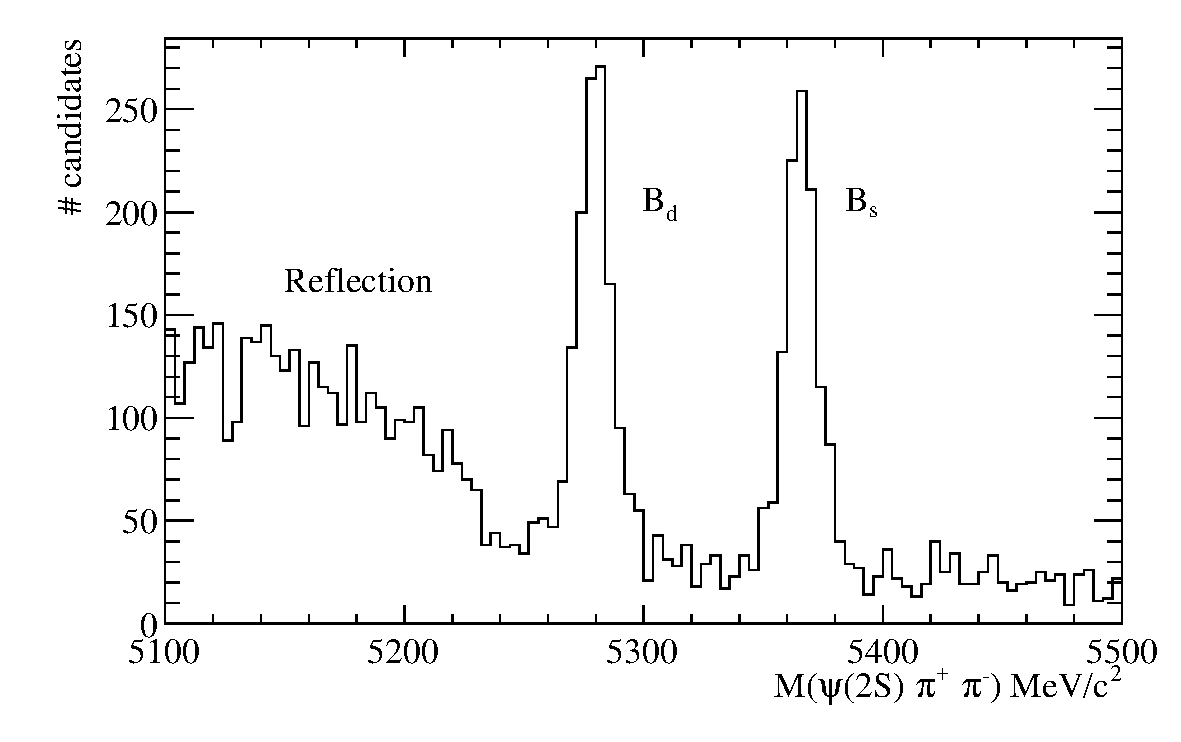
\includegraphics[width=0.75\textwidth]{figs/psi2Spipi.pdf}\\
%\caption
{\small $\psi ({\rm 2S}) \pi^{+} \pi^{-}$  invariant mass distribution.}
%\label{fig:bmass}
\end{center}
%\end{figure}
%


\begin{enumerate}


\item Consider first the $B_s$ peak which is the particle with the highest
mass, i.e. the right most peak in the plot. Construct a composite probability density
function (PDF) for the invariant mass of the muon pairs, which
contains two components :

\begin{itemize}
\item A Gaussian shape to fit the $B_s$ peak;
\item A shallow falling exponential to fit the background shape of the mass spectrum
underneath the peak.
\end{itemize}

\item Use this PDF in a Maximum Likelihood fit to determine the parameters of the PDF.
Note hat it is essential that the composite PDF remains normalised to 1 over the range
of the fit. 

Determine the $B_s$ meson mass and yield, and all other parameters, and their and
errors.

You should be able to obtain the parameter errors directly from the minimization engine of your choice (scipy.optimize.minimise, scipy.optimise.curve\_fit, lmfit, see \url{https://lmfit.github.io/lmfit-py/} or Minuit). Depending on your choice you will be able to chose different minimising methods.
It would be good to show that you understand these by obtaining them yourself from the parameters of the Gaussian signal fit - this is described in the data handling lectures.

Plot the fitted signal shape on top of the data.

\item Now consider the mass range above the reflection, and perform a simultaneous fit for both
peaks, and the underlying background. Again you should always report the parameter
values, and their errors. Plot the fitted signal shape on top of the data.

\item The results so far probably look "quite good" by eye.  i.e. the signal shape plotted on top of the data probably looks like it fits quite well.  However this can be misleading when performing a precision measurement.  You should make a plot of what are called the "residuals". A residual is the difference between the data in the binned histogram and the best-fit mass model value for the centre of that bin. Describe what you see.

\newpage

\item There are several ways to enhance the scope of the project.

\begin{itemize} 
\item For example, if the single
Gaussian mass model does not fit the data perfectly, one can try other mass models,
i.e. by using a signal PDF that goes beyond a single Gaussian
function. One example: is a PDF comprising a function which is the sum of two Gaussian functions (i.e. one
narrow and one wide Gaussian function to fit a single D meson
peak. Alternatively try a Crystal Ball function, which incorporates a non-Gaussian tail at the lower end of
the mass peak. The functional shape is described elsewhere, e.g. see:
\begin{verbatim}
https://en.wikipedia.org/wiki/Crystal_Ball_function 
\end{verbatim} 
You could implement each of these functions in your PDF and see how much better
they are at describing the data.
\item Try to extend the fit to include the kinematic reflection
\item Read the publication and see what is said about systematic errors. Make a reasonable
attempt at determining some systematic errors on the masses.
\item Compare your results to the PDG and previous measurements.
\item From the yields of $B_s$ and $B^0$ mesons, following the
  procedures in the papers try to evaluate the ratio of branching
  ratios of these modes.
\end{itemize}


\end{enumerate}

\subsection{Project planning}

The project descriptions are generally significantly less detailed than what was made available for the checkpoints. Any material covered during checkpoints including python code examples are assumed to be known.  Only essential and new information is provided and you are expected to take care of the details. Python code snippets are provided where necessary, but you will have to understand yourself what they do. It is recommend that you google for information about your project on the web, including data sheets of components and python libraries, if applicable. Python scripts should be well structured, either using functions or classes.

The timeline will vary between different projects, but in general, it is recommended that you plan your work as follows:
\begin{itemize}
\item	weeks 7, 8 \& 9: 	Building your gadget and/or writing code for project;
\item	week 9, 10: 	Analysis of data or equivalent, prepare supplementary material;
\item	week 10, 11:	Finish writing of project report and prepare submission.
\end{itemize}
Note that you are advised to start writing your report as the project progresses. 

For guidance on report writing, how the projects will be assessed, plagiarism and the submission deadline, please consult the DAH course booklet and the DAH grade descriptors, available on Learn.

 

\newpage
\section{Project G: Building a Remote Sensing System}

\subsection{Goals of project}

You will develop a remote sensing system, similar to a weather station.
A WiFi \microcontroller will be used to acquire temperature and humidity data
and publish these on a embedded web server. You will use the Raspberry-Pi to
download these data and build a monitoring system.


The projects have an open-ended aspect and are an opportunity where you can show your own initiative and demonstrate your experimental and computational skills. 


\subsection{Equipment for project G}

For this project you will need the following items:
\begin{itemize}
\item Raspberry-Pi
\item Adafruit HUZZAH ESP8266 WiFi  \microcontroller
\item DHT22 Temperature Humidity Sensor 
\item DC power supply
\item USB  to TTL UART 6PIN CP2102 Module Serial Converter
\item Adafruit RGB 16x2 LCD and Keypad Kit 
%\item ADAFRUIT INDUSTRIES  1112  STACKING HEADER
%\item ADAFRUIT INDUSTRIES  914  PI COBBLER BREAKOUT KIT
\item Windows PC in laboratory
\item WiFi hotspot 
%\item USB to WiFi adapter Wi-PI
\end{itemize}
Some of this equipment will be located in the red box G. You will have to share some items between Tuesday and Thursday sessions. 


\subsection{Building the Remote Sensing System}

You will develop a remote sensing system, similar to a weather station.
For this you need to put together different elements, including 
connecting a temperature and humidity sensor to a \microcontroller, 
programming the \microcontroller,
connecting an LCD display to the Raspberry-Pi,
and remotely connecting the sensing system to the Raspberry-Pi via
a WiFi hotspot. It is suggested that you familiarise yourself with all the components
by consulting the corresponding web pages and reading their  technical specifications.
A \microcontroller is a small computer on a single integrated circuit containing a processor core, memory, and programmable input/output peripherals,  so it is more limited than a 
Raspberry-Pi. Here we will use the Adafruit HUZZAH ESP8266 WiFi  \microcontroller,
see \url{https://learn.adafruit.com/adafruit-huzzah-esp8266-breakout/overview}.

\begin{enumerate}

\item Mount the Huzzah ESP8266 \microcontroller on a breadboard. 
Use a DC power supply to provide the +5V. 
Please note that it is always recommended to switch off the power supply when connecting devices or changing the wiring.
Connect the 3.3V output and GND to the rails on the breakout board. 
Then use the USB  to Serial cable - Receive, Transmit and Ground Lines (Rx,TX, GND) -
to connect the ESP8266 with to the Windows PC, 
located on the desk in the right-hand corner of the DAH laboratory. 
When connected, reset  theESP8266 by  pushing the
reset button while holding the GIPO0 button. 
This will make the \microcontroller ready to boot 
and a dimmed red LED will show.

\item To program the  ESP8266  you need to start the Arduino-IDE package, 
which is installed on the Windows PC. Using the instructions on
\url{https://learn.adafruit.com/adafruit-huzzah-esp8266-breakout/using-arduino-ide},
go to Arduino $\rightarrow$ File $\rightarrow$ Preferences and copy the following link into
the Additional Board Manager URLs field: 
\hspace*{5mm} {\tt http://arduino.esp8266.com/stable/package\_esp8266com\_index.json}\\
Then you invoke  the Board Manager (Tools $\rightarrow$ Board $\rightarrow$ Boards Manager),
search for say "ESP" and install "esp8266 by ESP8266 Community".
If successful, the  ESP8266 should appear under Tools $\rightarrow$ Board. 
Check that the CPU Frequency is set correctly (80 MHz) on the \microcontroller
and set upload baud rate (115200)  and the matching port of your USB to serial cable (e.g. COM4).

In addition you need to install two libraries.
Use the library manager (Sketch $\rightarrow$  Include Libraries $\rightarrow$ Library Manager), first  search for  say "Adafruit Unified" and install "Adafruit Unified Sensor library by Adafruit" then search for say "DHT" and install "DHT sensor library by Adafruit".
%There is one more step. You need to replace the file {\tt libm.a} from the following path,\\
%\hspace*{5mm}{\tt C:$\backslash$Users$\backslash<$username$>\backslash$AppData$\backslash%$Roaming$\backslash$Arduino15$\backslash$packages$\backslash$esp8266$\backslash$tools\\
%\hspace*{5mm}$\backslash$xtensa-lx106-elf-gcc$\backslash$1.20.0-26-gb404fb9$\backslash$xtensa-lx106-elf$\backslash$lib}\\ with a file with the same name, available from  \url{https://github.com/fmuheim/DAH}. 


\item As a first  programming exercise, perform the "Blink Test". Consult the instructions on
{\tt .../using-arduino-ide}.
Copy the code into an Arduino IDE sketch, compile the code (Sketch $\rightarrow$ Verify / Compile) and upload ($\Rightarrow$) to the \microcontroller. 
The sketch will start immediately - you'll see the LED blinking. Hooray!

\item The next step is to connect the temperature and humidity sensor DHT22, see \url{http://www.adafruit.com/products/385}, to the \microcontroller. The DHT22 requires  three lines (3.3V, GND and data). Use GPIO \#2 as serial input on the ESP8266. Remember to switch off the power supply during this process.


\item You are now ready to program the temperature and humidity web server. 
Download the example code into the Arduino-IDE application, using the instructions from \url{https://learn.adafruit.com/esp8266-temperature-slash-humidity-webserver/code}. \\
You will need to change this code by adding the name and password of the WiFi hotspot.
%
\lstinputlisting{../scripts/wifi.ino}
%
Compile the code (Sketch $\rightarrow$ Verify / Compile) and upload it
to the \microcontroller.  Recall to put first the \microcontroller ready into boot state.

\item In order to connect the ESP8266 \microcontroller to the WiFi hotspot, which  is located on the desk in the left corner of the laboratory, switch on the WiFi hotspot, if necessary, push the reset button on the \microcontroller and 
open a Serial Monitor on the  Arduino-IDE  ($\rightarrow$ Tools  $\rightarrow$ Serial monitor).
The ESP8266 \& DHT22 sensor system should start to work 
and you  should  obtain the IP address of the HTTP server, see:
\begin{verbatim}
    Working to connect ................................................................................................

    DHT Weather Reading Server
    IP Address: 192.168.1.2
    HTTP server  started
\end{verbatim}

\item The final step is to read the DHT22 \& ESP8266 remotely 
with the on-board WiFi adapter of  the Raspberry-Pi. To enable WiFi on the Raspberry-Pi,
execute the following command:
%
\begin{verbatim}
    studentnn@dahpimm  ~ $ wpa_cli enable wlan0 
\end{verbatim}
%
   Check the network connection and select the WiFi hotspot. You might have to type in the password. Using the Chromium web browser, you can now read the sensor by connecting to the correct IP address, e.g. {\tt http://192.168.1.2}.
Find out how to read temperature and humidity from the DHT22 Adafruit webpage, 
\url{https://learn.adafruit.com/esp8266-temperature-slash-humidity-webserver/using-the-webserver}.

 
\end{enumerate}

\subsection{Using the  Remote Sensing System}

Reading temperature and humidity using a web browser is 
straightforward, but you want to go beyond single measurements.
Write a python script which samples a series of measurements
and displays these. For this you need to parse the web server data.
Use the instructions at
%\url{http://www.diveintopython.net/html_processing/extracting_data.html} 
% \url{http://stackoverflow.com/questions/2792650/python3-error-import-error-no-module-name-urllib2}
https://docs.python.org/3/howto/urllib2.html
to write a script that will regularly read the temperature and humidity from
the remote sensor and print the data onto the screen and/or file. What would be a reasonable
update frequency? Further possible applications could include the following:

\begin{enumerate}

\item Write a  well structured python script in which reading the temperature and humidity sensor are
functions or classes.  Convert temperature values from Fahrenheit into Celsius.

\item Write a script which displays an animated series of measurements in real time.
Use a hot air-blower/hair-dryer to vary the temperature. 
Avoid applying the heat-source for too long to prevent the DHT22 from starting to melt.
Plot the temperature versus humidity 
and explain what you observe.
 
\item Display the temperature and humidity on an  LCD display. 
Connect the LCD display to top of the Raspberry-Pi. 
Make sure that you use the provided GPIO port Extender plug to keep the LCD board from touching the  USB and Ethernet ports of the Raspberry-Pi. 
Download the python script {\tt  char\_lcd\_plate.py} from  \url{https://github.com/fmuheim/DAH}. Run this script to understand how to program the LCD display. Consulting the instructions at \\
\url{https://learn.adafruit.com/adafruit-16x2-character-lcd-plus-keypad-for-raspberry-pi/usage}, 
write a python script which regularly reads  and updates temperature (in Celsius) and humidity 
on the LCD display.

\end{enumerate}


\begin{comment}
\begin{verbatim}

convert temperature to Celsius



python scripts 
	RemoteTemp.py will be given
	make animated plot
	drive LCD screen

use hairdryer

\end{verbatim}


\begin{verbatim}
connect DHT22  to ESP8266 
connections
Sensor: DHT22: 
	power 3.3V, Gnd, serial
micro-controller ESP8266 
	Power V+ 5V
	GND
	GPIO use #2 as serial input
	3.3V output to rail
	communication Tx, Rx and Gnd
Connect via USB-serial (CP2102) to Windows PC

program the micro-controller using Arduino-IDE on the Windows PC
example code on
https://learn.adafruit.com/esp8266-temperature-slash-humidity-webserver/code
	Need to set password, ...
do blink test first
	https://learn.adafruit.com/adafruit-huzzah-esp8266-breakout/using-arduino-ide
open Arduino-IDE -> Tools -> Serial monitor
to get status and IP address

need to decide, if we do this.

WiFi hotspot - plug in, switch on
 
Raspberry-Pi
establish connection, (might need Pi account)

Webbrowser
IP address
read some sample

connect LCD screen to Raspberry Pi using I2C

description
	builds a circuit with sensor  and ESP8266,
	needs 5 V power supply
	student/supervisor programs arduino via USB serial using PC
	ESP8266 connects to Wifi hotspot 
	wifi hotspot has password
	Raspberry pi connect to wifi hotspot via USB/Wifi	
	Student opens browser on raspberry
	go to wifi address of  ESP8266

write script in python go get temp/humid measurements,
get data continuously,
plot these (animated), similar to fft or temp sensor project
time interval 2 to 3 s.?
	
\end{verbatim}

%\subsection{Performing Remote Sensing and Analysis}



\begin{verbatim}

convert temperature to Celsius



python scripts 
	RemoteTemp.py will be given
	make animated plot
	drive LCD screen

use hairdryer

\end{verbatim}
\end{comment}

\subsection{Project planning}

The project descriptions are generally significantly less detailed than what was made available for the checkpoints. Any material covered during checkpoints including python code examples are assumed to be known.  Only essential and new information is provided and you are expected to take care of the details. Python code snippets are provided where necessary, but you will have to understand yourself what they do. It is recommend that you google for information about your project on the web, including data sheets of components and python libraries, if applicable. Python scripts should be well structured, either using functions or classes.

The timeline will vary between different projects, but in general, it is recommended that you plan your work as follows:
\begin{itemize}
\item	weeks 7, 8 \& 9: 	Building your gadget and/or writing code for project;
\item	week 9, 10: 	Analysis of data or equivalent, prepare supplementary material;
\item	week 10, 11:	Finish writing of project report and prepare submission.
\end{itemize}
Note that you are advised to start writing your report as the project progresses. 

For guidance on report writing, how the projects will be assessed, plagiarism and the submission deadline, please consult the DAH course booklet and the DAH grade descriptors, available on Learn.




\newpage
\section{Project X: Develop a Project or Suggest Your Own Project}

\subsection{Goals of project}

We have a few possible projects where the project descriptions and goals are not advanced enough to be included in the list of projects A to G, see the list below. If you are interested in one of these, please let us know. In addition, if you have an idea of what you want to do with the Raspberry-Pi, please tell us and we will discuss it. Please note that we will have to make a decision if your own project or one from the list below is feasible within the time scale of the DAH course.


\subsection{List of possible projects}

We give here a list of projects using the Raspberry-Pi and/or the Arduino, where more development work is required and little or no project description exists. 

\begin{itemize}
\item Building an oscilloscope using the Arduino micro-controller as an ADC and the Raspberry-Pi as the DAQ to display waveforms.
\item Building a motion sensor using an accelerometer connected to an ADC and read out by the Raspberry Pi.
\item Build a CCTV-like imaging capturing triggered by a motions sensor, for info see 
\url{http://www.raspberrypi.org/learning/python-picamera-setup/}.
\item Control switches, LEDs and relays using the PiFace Digital expansion boards, see 
\url{http://www.piface.org.uk/products/piface_digital/}.
\item Controlling a toy train set-up in the laboratory, for info see the following web link: 
\url{http://www.mathworks.co.uk/company/newsletters/articles/adding-fun-to-first-year-computer-programming-classes-with-matlab-arduino-microcontrollers-and-model-trains.html?nocookie=true}.
You will need to bring your own toy train set-up.
\item Suggest your own project.
\end{itemize}

\subsection{Project planning}

The project descriptions are generally significantly less detailed than what was made available for the checkpoints. Any material covered during checkpoints including python code examples are assumed to be known.  Only essential and new information is provided and you are expected to take care of the details. Python code snippets are provided where necessary, but you will have to understand yourself what they do. It is recommend that you google for information about your project on the web, including data sheets of components and python libraries, if applicable. Python scripts should be well structured, either using functions or classes.

The timeline will vary between different projects, but in general, it is recommended that you plan your work as follows:
\begin{itemize}
\item	weeks 7, 8 \& 9: 	Building your gadget and/or writing code for project;
\item	week 9, 10: 	Analysis of data or equivalent, prepare supplementary material;
\item	week 10, 11:	Finish writing of project report and prepare submission.
\end{itemize}
Note that you are advised to start writing your report as the project progresses. 

For guidance on report writing, how the projects will be assessed, plagiarism and the submission deadline, please consult the DAH course booklet and the DAH grade descriptors, available on Learn.



 

